\documentclass{article}

\usepackage{graphicx}
\usepackage{gensymb}

\begin{document}
\newpage
   \vspace*{\stretch{1.0}}
   \begin{center}
      \Large\textbf{Earth 270 Disaster Report: 526 Antioch Earthquake}\\
      \large\textit{John Lawson}
   \end{center}
   \vspace*{\stretch{2.0}}

\newpage

\section{Introduction}
 The 526 Antioch Earthquake was a major disaster which occurred in late May of
 526 AD, near the city of Antioch (Sbeinati et al, 2005). The death toll was 
 increased by the influx of visitors to the city for a religious festival, causing
 an estimated 250000 to 300000 casualties (Glanville et al, 1958).\\
 
 %\ref{fig:rawData}.\\

\newpage 
\section{Context Of The Disaster}
 The city of Antioch was located in northern Palestine, near the modern day city
 of Antakya in Turkey. Its exact location was roughly 36 degrees 12 minutes N,
  and 36 degrees 10 minutes E (tools.wmflabs.org, 2018).
 The region is located near a transform plate boundary between the Arabian and
 African plates (Hempton, 1987). Because of this tectonic instability, the region
 surrounding Antioch was considered prone to suffering heavy damage from
 earthquakes throughout its history (Sbeinati et al, 2005). \\
 
 \begin{figure}[h]
	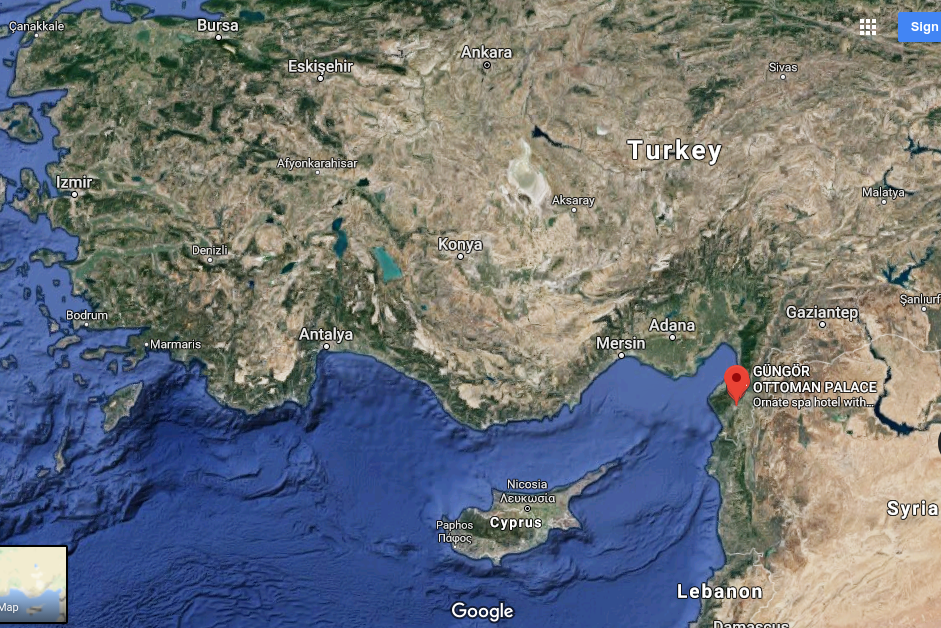
\includegraphics[width=\linewidth]{antiochMap.png}
	\caption{Location of modern Antakya, courtesy of Google Maps}
	\label{fig:antakyaMap}
 \end{figure}
\newpage
\section{The Disaster}
 Sometime between May 20th and May 29th of 526 AD, the city of Antioch was struck
 by an earthquake which caused extensive damage. According to John of Ephesus,
 the earthquake began on the 7th hour of the day, damaging many buildings which
 were subsequently consumed by fires that raged in the aftermath. Some observers
 reported evidence of chasms opening up in the earth in the area, as well as
 relative movement of the ground outside of the city. Liquefaction of soil was
 observed as well as a potential sighting of a dubious phenomenon known as
 Earthquake Lights (Sbeinati et al, 2005). The reported sightings of Earthquake
 Lights may have simply been misinterpreted references to the burning city itself (Stothers, 2004).

\section{Analysis}
 The severity of the disaster was amplified by the coincidental timing of a large
 influx of visitors to the city, as well as the relative intensity of the event,
 estimated as a 7.0 on the Richter Scale (Sbeinati et al, 2005). Given the era
 of the disaster, little reliable warning would have been available to prepare
 for the earthquake.

\newpage
\section{references}
(n.d.). Retrieved March 29, 2018, from https://tools.wmflabs.org/geohack/geohack.php\\
Sbeinati, M. R., Darawcheh, R., \& Mouty, M. (2005). The historical earthquakes of Syria: an analysis of large and moderate earthquakes from 1365 BC to 1900 AD. Annals of Geophysics, 48(3).\\
Hempton, M. R. (1987). Constraints on Arabian plate motion and extensional history of the Red Sea. Tectonics, 6(6), 687-705.\\
Downey, G. (1958, January). The size of the population of Antioch. In Transactions and Proceedings of the American Philological Association (Vol. 89, pp. 84-91). Johns Hopkins University Press, American Philological Association.\\
Stothers, R. B. (2004). Ancient and modern earthquake lights in northwestern Turkey. Seismological Research Letters, 75(2), 199-204.\\	

\end{document}
